\section{Introduction}
\label{sec:introduction}

% state the learning objective 

\par The objective of this laboratory assignment is to study an RC circuit as described in Figure~\ref{fig:rc}.


\begin{figure}[h]
\centering
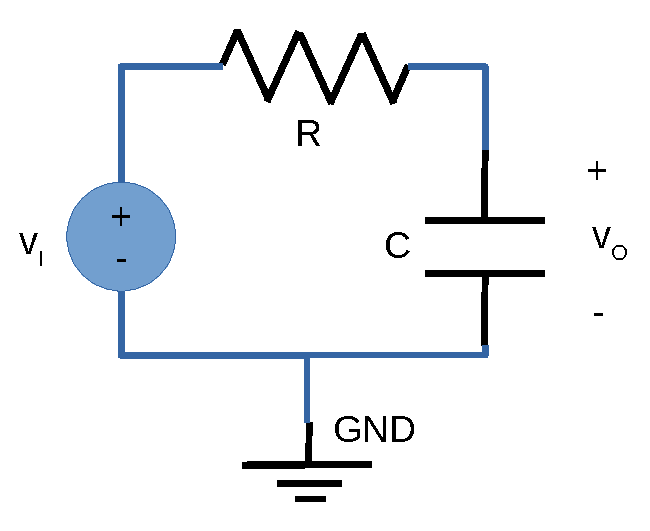
\includegraphics[width=0.9\linewidth]{../doc/rc.pdf}
\caption{T2 RC circuit.}
\label{fig:rc}
\end{figure}


\par In Section~\ref{sec:analysis}, a theoretical analysis of the circuit is made, by applying different methods, such as the Thevenin and Phasor analysis, and the total solution (natural plus forced solutions) of the circuit is presented. The theoretical frequency response of the circuit is also presented in this section. In Section~\ref{sec:simulation}, the circuit is analysed by simulation in NGSpice and the results obtained for the operating point and transient analysis are compared to the theoretical results obtained in Section~\ref{sec:analysis}. The conclusions of this study are outlined in Section~\ref{sec:conclusion}.

$NOTE:$~This report was automatically generated. The data used was supplied by inputting 95780 to the $t2\_datagen.py$ file. A different set of data should automatically yield coherent results.

